\documentclass[12pt, oneside, a4]{report}
%%% Packages
%%      NOTE:   Do not edit any predefined packages.
%%              Contact author if necessary.
\usepackage{graphicx}
\usepackage{lipsum}
\usepackage{geometry}
\geometry{
    left    = 40mm,
    right   = 25mm,
    top     = 25mm,
    bottom  = 25mm,
    a4paper
}
%\usepackage[none]{hyphenat}
\usepackage{times}
\usepackage{appendix}
\usepackage{ifthen}
\usepackage{lastpage}
\usepackage{setspace}
\usepackage{tocloft}
\usepackage{titlesec}
\usepackage{nomencl}
\usepackage{etoolbox}
\usepackage{siunitx}
\usepackage{amsfonts, amsmath, amssymb, amsthm}
\usepackage[justification=centering,position=top]{caption}
\usepackage{tikz, circuitikz, smartdiagram}
\usepackage{hologo}
\usepackage{parskip}

%% Test packages
\usepackage[grid, gridunit=mm, gridcolor=blue!40, subgridcolor=blue!20]{eso-pic}
\usepackage{showframe}

%% Add more required packages after this line



%%% Main graphical rules and styling formats
\titleformat{\chapter}[display]
    {\bfseries\normalsize}
    {\centering CHAPTER \thechapter}
    {48pt}
    {\centering\normalsize\uppercase}
\titlespacing*{\chapter}{0pt}{-28pt}{48pt}

\titleformat{\section}
    {\bfseries\normalsize}
    {\thesection.}
    {10mm}
    {\normalsize}
\titlespacing*{\section}{0pt}{24pt}{12pt}

\titleformat{\subsection}
    {\bfseries\normalsize}
    {\thesubsection.}
    {10mm}
    {\normalsize}
\titlespacing*{\subsection}{0pt}{24pt}{12pt}

\titleformat{\subsubsection}
    {\bfseries\normalsize}
    {\thesubsubsection.}
    {10mm}
    {\normalsize}
\titlespacing*{\subsubsection}{0pt}{24pt}{12pt}

\captionsetup[table]{labelsep=space, skip=12pt}
\captionsetup[figure]{labelsep=space, skip=24pt}
\DeclareCaptionFont{mysize}{\normalsize}
\captionsetup{font=mysize}

%%% Macros
\newcommand{\signaturespace}[3]
    {
        \hfill\parbox[t][0pt]{60mm}
        {\rule{#3}{.5pt}\\\centering #1\\#2}
    }

\newcommand{\cosignaturespace}[3]
    {
        \parbox[t][0pt]{60mm}
        {\rule{#3}{.5pt}\\\centering #1\\Co-Supervisor}
        \hfill
        \parbox[t][0pt]{60mm}
        {\rule{#3}{.5pt}\\\centering #2\\Supervisor}
    }

\newcommand{\addmember}[4]
    {
        \vspace{12pt}
        #1\\#2 \hfill \rule{#4}{.5pt}\\#3
    }


%%% User definitions
\def\thesisname{This is the thesis name and it is not essential to be in uppercase or lowercase}
\def\thesisnameTR{THis is the thesis name translated in Turkish}
\def\surname{Surname}
\def\firstname{Name}
\def\degreeshort{PhD} % MS, ARCH, or PhD
\def\deptname{Electrical-Electronics Engineering} % The full name of the dept.
\def\mainFOS{Electrical-Electronics Engineering} % The full name of the main field of study
\def\deptnameTR{Elektrik-Elektronik Mühendisliği} % The full name of the dept. in Turkish
\def\mainFOS{Elektrik-Elektronik Mühendisliği} % The full name of the main field of study in Turkish
\def\thesisMonth{July} % The corresponding month of the thesis
\def\thesisYear{2023} % The corresponding year of the thesis
\def\thesisMonthTR{Temmuz} % The corresponding monthe of the thesis in Turkish
\def\directortitlename{Prof. Dr. Name SURNAME} % The title and the name of the director
\def\headofdepttitlename{Prof. Dr. Name SURNAME} % The title and the name of the head of the department
\def\supervisorname{Assoc. Prof. Yaser DALVEREN} % The title and the name of the supervisor
\def\cosupervisorname{Assoc. Prof. Enver ÇAVUŞ} % The title and the name of the co-supervisor
\def\supervisornameTR{Doç. Dr. Yaser DALVEREN} % The title and the name of the supervisor
\def\cosupervisornameTR{Doç. Dr. Enver ÇAVUŞ} % The title and the name of the co-supervisor
\def\defensedate{\today} % Defense date in dd MMM, yyyy format
\def\dedication{my wife,\\who has been my most profound inspiration.} % Dedication of this thesis

\ifthenelse{\equal{\degreeshort}{MS}}
    {\def\degreelong{Master of Science}
     \def\degreeshortTR{Yüksek Lisans}}
    {% else1
    \ifthenelse{\equal{\degreeshort}{ARCH}}
        {\def\degreelong{Architecture}
         \def\degreeshortTR{Mimarlık}}
        {% else2
            \ifthenelse{\equal{\degreeshort}{PhD}}
            {\def\degreelong{Doctor of Philosophy}
             \def\degreeshortTR{Doktora}}
            {% else3
                \def\degreelong{PLEASE CHECK THE DEFINITION of degreeshort AND CORRECT IT}
}}}
\ifthenelse{\equal{\degreeshort}{ARCH}}{\def\aan{AN}}{\def\aan{A}}
\def\namesurname{\firstname~\surname}

\begin{document}
\sloppy
\singlespacing

\pagenumbering{roman}
\thispagestyle{empty}
% 
~\vspace{35mm}
\begin{center}
    \MakeUppercase{\thesisname}
    
    \vspace{96pt}
    THE GRADUATE SCHOOL OF NATURAL AND APPLIED SCIENCES \\ OF \\ ATILIM UNIVERSITY

    \vspace{132pt}
    \MakeUppercase{\namesurname}

    \vspace{60pt}
    \aan~\MakeUppercase{\degreelong} THESIS\\IN\\
    THE DEPARTMENT OF \MakeUppercase{\deptname}\\(MAIN FIELD OF STUDY: \MakeUppercase{\mainFOS})

    \vfill
    \MakeUppercase{\thesisMonth~\thesisYear}

\end{center}
\newpage
\thispagestyle{empty}
~\vspace{35mm}
\begin{center}
    \MakeUppercase{\thesisname}

    \vspace{84pt}
    A THESIS SUBMITTED TO\\THE GRADUATE SCHOOL OF NATURAL AND APPLIED SCIENCES\\OF\\ATILIM UNIVERSITY
    
    \vspace{12pt}
    BY

    \vspace{12pt}
    \MakeUppercase{\namesurname}

    \vspace{96pt}
    IN PARTIAL FULFILLMENT OF THE REQUIREMENTS\\FOR\\THE DEGREE OF \MakeUppercase{\degreelong}\\IN\\THE DEPARTMENT OF \MakeUppercase{\deptname}\\(MAIN FIELD OF STUDY: \MakeUppercase{\mainFOS})

    \vfill
    \MakeUppercase{\thesisMonth~\thesisYear}
\end{center}
\newpage
\thispagestyle{empty}
\setlength{\parindent}{0mm}

Approval of the Graduate School of Natural and Applied Sciences, Atilim University.

\vspace{24pt}

\signaturespace{\directortitlename}{Director}{60mm}

\vspace{24pt}


\vspace{48pt}
I certify that this thesis satisfies all the requirements as a thesis for the degree of {\bfseries \degreelong~in \deptname, Atilim University}.

\vspace{24pt}

\signaturespace{\headofdepttitlename}{Head of Department}{60mm}

\vspace{48pt}

This is to certify that we have read the thesis \MakeUppercase{\thesisname} submitted by \MakeUppercase{\namesurname} and that in our opinion it is fully adequate, in scope and quality, as a thesis for the degree of Master of Science- Architecture/Doctor of Philosophy.

\vspace{24pt}

\cosignaturespace{\cosupervisorname}{\supervisorname}{60mm}

\vspace{60pt}

{\bfseries Examining Committee Members:}
\vspace{12pt}

\addmember{Prof. Dr. Committee MEMBER I}{Electrical-Electronics Eng. Dept.}{Testname University}{60mm}

\addmember{Prof. Dr. Committee MEMBER II}{Computer Eng. Dept.}{Testname University}{60mm}

\addmember{Prof. Dr. Committee MEMBER III}{Biomedical Dept.}{Testname University}{60mm}

%%      Note: Uncomment below if committee member IV and V exist.
%\addmember{Prof. Dr. Committee MEMBER I}{Electrical-Electronics Eng. Dept.}{Testname University}{60mm}

%\addmember{Prof. Dr. Committee MEMBER I}{Electrical-Electronics Eng. Dept.}{Testname University}{60mm}

\newpage
\thispagestyle{empty}

\hfill {\bfseries Date: }\defensedate

\newpage
\thispagestyle{empty}
~

\vspace{120mm}
I hereby declare that all information in this document has been obtained and presented in accordance with academic rules and ethical conduct. I also declare that, as required by these rules and conduct, I have fully cited and referenced all material and results that are not original to this work.

\vspace{30mm}
\hfill Name, Last Name:\hspace{40mm}

\vspace{10mm}
\hfill Signature:\hspace{40mm}

\newpage
\setcounter{page}{3}
\onehalfspacing % One and half spacing
\addcontentsline{toc}{subparagraph}{ABSTRACT}
\begin{center}
    {\bfseries ABSTRACT

    \vspace{48pt}
    \MakeUppercase{\thesisname}}

    \vspace{24pt}
    \surname, \firstname

    \degreeshort., Department of \deptname

    Supervisor: \supervisorname
    
    Co-Supervisor: \cosupervisorname

    \vspace{24pt}
    \thesisMonth~\thesisYear, \pageref{LastPageLabel}~pages
\end{center}

\vspace{48pt}
Write the abstract text here. \lipsum[1]

\vspace{48pt}
Keywords: Write keywords here.
\newpage
\addcontentsline{toc}{subparagraph}{ÖZ}

\begin{center}
    {\bfseries ÖZ

    \vspace{48pt}
    \MakeUppercase{\thesisnameTR}}

    \vspace{24pt}
    \surname, \firstname

    \degreeshortTR, \deptnameTR~Bölümü

    Tez Yöneticisi: \supervisornameTR
    
    Ortak Tez Yöneticisi: \cosupervisornameTR

    \vspace{24pt}
    \thesisMonthTR~\thesisYear, \pageref{LastPageLabel}~sayfa
\end{center}

\vspace{48pt}
Tezin Türkçe özeti buraya yazılacak. \lipsum[1]

\vspace{48pt}
Anahtar kelimeler: Anahtar kelimelerin Türkçelerini buraya yazın.

% Dedication
\newpage
\addcontentsline{toc}{subparagraph}{DEDICATION}
~
\vfill

\begin{center}
    \textit{To \dedication}
\end{center}
\vfill

% Acknowledgements
\newpage
\addcontentsline{toc}{subparagraph}{ACKNOWLEDGEMENTS}

\begin{center}
    {\bfseries ACKNOWLEDGEMENTS}
\end{center}

\vspace{24pt}
I would like to express ...

I shall also thank to ...

Furthermore, I thank the members of ...

The financial support of The Scientific and Technical Research Council of Turkey
(TUBITAK) is also acknowledged.

Finally, ...

% TOC
\newpage
\renewcommand{\contentsname}{\normalsize TABLE OF CONTENTS}
\renewcommand{\cfttoctitlefont}{\hfill\Large\bfseries}
\renewcommand{\cftaftertoctitle}{\hfill~}
\setlength{\cftbeforetoctitleskip}{-18pt}
\setlength{\cftaftertoctitleskip}{36pt}

\setlength{\cftbeforechapskip}          {0pt}
\setlength{\cftbeforesecskip}           {0pt}
\setlength{\cftbeforesubsecskip}        {0pt}
\setlength{\cftbeforesubsubsecskip}     {0pt}
\setlength{\cftbeforeparaskip}          {0pt}

\setlength{\cftchapindent}              {.25in}
\setlength{\cftsecindent}               {.5in}
\setlength{\cftsubsecindent}            {.75in}
\setlength{\cftsubsubsecindent}         {1in}
\setlength{\cftparaindent}              {0mm}
\setlength{\cftsubparaindent}              {0mm}

\setlength{\cftchapnumwidth}            {0em}
\setlength{\cftsecnumwidth}             {0em}
\setlength{\cftsubsecnumwidth}          {0em}
\setlength{\cftsubsubsecnumwidth}       {0em}

%% Indents
\renewcommand{\cftchapaftersnumb}{\hspace{.25in}}
\renewcommand{\cftsecaftersnumb}{\hspace{.25in}}
\renewcommand{\cftsubsecaftersnumb}{\hspace{.5in}}
\renewcommand{\cftsubsubsecaftersnumb}{\hspace{.75in}}

%% Dotsep
\renewcommand\cftdotsep{0.1}
\renewcommand{\cftchapleader}{\cftdotfill{\cftdotsep}}
\renewcommand{\cftsecleader}{\cftdotfill{\cftdotsep}}
\renewcommand{\cftsubsecleader}{\cftdotfill{\cftdotsep}}
\renewcommand{\cftsubsubsecleader}{\cftdotfill{\cftdotsep}}

%% Chapter rearrangement
\renewcommand{\cftchappresnum}{}
\renewcommand{\cftchapaftersnum}{.~}
\renewcommand{\cftchapfont}{\normalsize\MakeUppercase{}}
\renewcommand{\cftchappagefont}{}

%% Paragraph rearrangement
\renewcommand{\cftparafont}{}
\renewcommand{\cftparaleader}{~}
\renewcommand{\cftparapagefont}{}

\setcounter{tocdepth}{6}
\setcounter{secnumdepth}{6}

\makeatletter
\let\old@l@paragraph\l@paragraph
\renewcommand{\l@paragraph}[2]{\old@l@paragraph{#1}{}}
\makeatother








\let\origaddvspace\addvspace
\renewcommand{\addvspace}[1]{}









\renewcommand{\listtablename}{\normalsize LIST OF TABLES}
\renewcommand{\cftlottitlefont}{\hfill\Large\bfseries}
\renewcommand{\cftafterlottitle}{\hfill~}
\setlength{\cftbeforelottitleskip}{-18pt}
\setlength{\cftafterlottitleskip}{36pt}
\renewcommand{\cfttabpresnum}{Table~}
\setlength{\cftbeforetabskip}{0pt}
\setlength{\cfttabindent}{0mm}
\setlength{\cfttabnumwidth}{5.5em}









\renewcommand{\listfigurename}{\normalsize LIST OF FIGURES}
\renewcommand{\cftloftitlefont}{\hfill\Large\bfseries}
\renewcommand{\cftafterloftitle}{\hfill~}
\setlength{\cftbeforeloftitleskip}{-18pt}
\setlength{\cftafterloftitleskip}{36pt}
\renewcommand{\cftfigpresnum}{Figure~}
\setlength{\cftbeforefigskip}{0pt}
\setlength{\cftfigindent}{0mm}
\setlength{\cftfignumwidth}{5.5em}








\addcontentsline{toc}{subparagraph}{TABLE OF CONTENTS}

\tableofcontents

% LOT
\newpage

\addcontentsline{lot}{paragraph}{TABLES}

\addcontentsline{toc}{subparagraph}{LIST OF TABLES}

\listoftables

% LOF
\newpage
\addcontentsline{toc}{subparagraph}{LIST OF FIGURES}

\addcontentsline{lof}{paragraph}{FIGURES\hfill}


\listoffigures

\renewcommand{\addvspace}[1]{\origaddvspace{#1}}

% List of symbols & abbreviations
\newpage
\addcontentsline{toc}{subparagraph}{LIST OF SYMBOLS/ABBREVIATIONS}
%%% Nomenclature items
\renewcommand{\nompreamble}{\vspace*{-10mm}}
\renewcommand\nomgroup[1]{%
\vspace{12pt}
  \item[\bfseries
  \ifstrequal{#1}{A}{Roman Letter Symbols}{%
  \ifstrequal{#1}{B}{Greek Letter Symbols}{%
  \ifstrequal{#1}{C}{Acronyms}{}}}%
]}
\renewcommand{\nomname}{\vspace{6pt}\centering\normalsize LIST OF SYMBOLS/ABBREVIATIONS\vspace{-20mm}\vspace{48pt}}

\newcommand{\nomunit}[1]{%
\renewcommand{\nomentryend}{\hspace*{\fill}#1}}
\makenomenclature

\setlength{\nomitemsep}{-\parsep}
%% Items in group A
\nomenclature[A]{$q$}{Finite Field Order}
\nomenclature[A]{$GF(q)$}{Finite Field of Order $q$}
\nomenclature[A]{$p$}{Prime Order of Base Finite Field}
\nomenclature[A]{$m$}{Finite Field Extension Factor}
\nomenclature[A]{$T$}{Faster-than-Nyquist Sampling Period
    \nomunit{\si{\second}}}
\nomenclature[A]{$T_0$}{Nyquist Sampling Period
    \nomunit{\si{\second}}}
\nomenclature[A]{$E_s$}{Symbol Energy
    \nomunit{\si{\joule}}}
\nomenclature[A]{$N_0$}{Noise Power Spectral Density
    \nomunit{\si{\watt\per\hertz}}}
\nomenclature[A]{$P_s$}{Signal Power
    \nomunit{\si{\watt}}}
\nomenclature[A]{$d_H$}{Hamming Distance}
\nomenclature[A]{$d_{min}$}{Minimum Hamming Distance}
\nomenclature[A]{$z_i$}{Result of the $i$th Syndrome}
\nomenclature[A]{$K_H$}{Message Vector Length}
\nomenclature[A]{$M_H$}{Parity Vector Length}
\nomenclature[A]{$N_H$}{Encoded Message Vector Length}
\nomenclature[A]{$H$}{Parity Check Matrix}
\nomenclature[A]{$G$}{Intersymbol Interference Matrix}
\nomenclature[A]{$E_b$}{Bit Energy
    \nomunit{\si{\joule}}}
\nomenclature[A$L$]{$\mathcal{L}$}{Configuration}
\nomenclature[A]{$S_C$}{Configuration Set}
\nomenclature[A]{$W_n$}{$n$-Dimensional Hadamard Matrix}
\nomenclature[A]{$n_m$}{Extended Min-Sum Truncation Size}
\nomenclature[A]{$n_b$}{Bubble Size}
\nomenclature[A]{$R$}{Code Rate}
\nomenclature[A]{$d_c$}{Check Node Depth}
\nomenclature[A]{$d_v$}{Variable Node Depth}
\nomenclature[A$Nm$]{$\mathcal{N}_m$}{Indices Connected to $m$th Check}
\nomenclature[A$Mn$]{$\mathcal{M}_n$}{Indices Connected to $n$th Variable}

%% Items in group B
\nomenclature[B$a$]{$\alpha$}{Primitive Element of Finite Field}
\nomenclature[B$b$]{$\beta$}{Roll-off Factor}
\nomenclature[B$c$]{$\gamma_A$}{Scalar Representing Neglected Likelihoods}
\nomenclature[B$l$]{$\lambda$}{Log-Likelihood Ratio}
\nomenclature[B$Os$]{$\Omega_s$}{Sampling Frequency
    \nomunit{\hspace{1mm}\si{\radian\per\second}}}
\nomenclature[B$On$]{$\Omega_N$}{Nyquist Frequency
    \nomunit{\si{\radian\per\second}}}
\nomenclature[B$w$]{$\phi$}{Offset of Min-Sum Approximation}
\nomenclature[B$s1$]{$\sigma$}{Noise Standard Deviation}
\nomenclature[B$s2$]{$\sigma^2$}{Noise Variance}
\nomenclature[B$t$]{$\tau$}{Time Acceleration Parameter}
\nomenclature[B$x$]{$\xi$}{Offset of Extended Min-Sum Algorithm}
\nomenclature[B$x0$]{$\xi_0$}{Initial Offset of Extended Min-Sum Algorithm}

%% Items in group C
\nomenclature[C]{AND}{Logical AND Operation}
\nomenclature[C]{APP}{A Posteriori Probability}
\nomenclature[C]{AWGN}{Additive White Gaussian Noise}
\nomenclature[C]{BCJR}{Bahl, Cocke, Jelinek and Raviv}
\nomenclature[C]{BER}{Bit Error Rate}
\nomenclature[C]{bit}{Binary Digit}
\nomenclature[C]{BP}{Belief Propagation}
\nomenclature[C]{BPSK}{Binary Phase Shift Keying}
\nomenclature[C]{BSC}{Binary Symmetric Channel}
\nomenclature[C]{C2V}{Check-to-Variable}
\nomenclature[C]{CD-ROM}{Compact Disc Read Only Memory}
\nomenclature[C]{ECC}{Error Correction Code}
\nomenclature[C]{ECN}{Elementary Check Node}
\nomenclature[C]{EMS}{Extended Min-Sum}
\nomenclature[C]{FB}{Forward-Backward}
\nomenclature[C]{FFT}{Fast Fourier Transform}
\nomenclature[C]{FTN}{Faster-than-Nyquist}
\nomenclature[C]{FPGA}{Field-Programmable Gate Array}
\nomenclature[C]{IFFT}{Inverse Fast Fourier Transform}
\nomenclature[C]{ISI}{Intersymbol Interference}
\nomenclature[C]{LDPC}{Low Density Parity Check}
\nomenclature[C]{LDR}{Log-Density Ratio}
\nomenclature[C]{LLR}{Log-Likelihood Ratio}
\nomenclature[C]{LUT}{Look Up Table}
\nomenclature[C]{M-BCJR}{\textit{M}-Algorithm Bahl, Cocke, Jelinek and Raviv}
\nomenclature[C]{NB-LDPC}{Nonbinary Low Density Parity Check}
\nomenclature[C]{NOO}{Number of Operations}
\nomenclature[C]{PCE}{Parity Check Equation}
\nomenclature[C]{PCM}{Parity Check Matrix}
\nomenclature[C]{PN}{Permutation Node}
\nomenclature[C]{PSD}{Power Spectral Density
    \nomunit{\si{\watt\per\hertz}}}
\nomenclature[C]{QPSK}{Quadrature Phase Shift Keying}
\nomenclature[C]{RAM}{Random Access Memory}
\nomenclature[C]{rRC}{Root-Raised-Cosine}
\nomenclature[C]{SE}{Spectral Efficiency}
\nomenclature[C]{SNR}{Signal-to-Noise Ratio
    \nomunit{\si{\decibel}}}
\nomenclature[C]{SPA}{Sum-Product Algorithm}
\nomenclature[C]{SSSgb\textit{K}SE}{Symbol-by-Symbol with go-back-\textit{K} Sequence Estimator}
\nomenclature[C]{SSSSE}{Successive Symbol-by-Symbol Sequence Estimator}
\nomenclature[C]{V2C}{Variable-to-Check}
\nomenclature[C]{WER}{Word Error Rate}
\nomenclature[C]{XOR}{Logical Exclusive OR Operation}

{\setlength{\parskip}{6pt}
\linespread{1}
\printnomenclature[25mm]}










\newpage
\setlength{\parskip}{8pt}
\setcounter{page}{1}
\pagenumbering{arabic}
\addcontentsline{toc}{paragraph}{CHAPTER}
% Thesis content goes here starting from the introduction
\chapter{INTRODUCTION}
\lipsum[1]
\section{Sample Introductory Subsection}
\lipsum[1-3]
\section{Another Subsection Goes Like This}
\lipsum[1-5]

\chapter{SECOND CHAPTER NAME}
\lipsum[1-3]
\section{Section Test}
\lipsum[1-10]
\section{Another Section to the Second Chapter}
\lipsum[1-4]

\begin{table}[h]
    \centering
    \caption{The first test table}
    \begin{tabular}{|c||c|c|}
        \hline
        \bfseries Name & \bfseries Category \#1 & \bfseries Category \#2 \\\hline\hline
        Testname 1 & Item 1.1 & Item 1.2\\\hline
        Testname 2 & Item 2.1 & Item 2.2\\\hline
        Testname 3 & Item 3.1 & Item 3.2\\\hline
    \end{tabular}
    \label{tab1}
\end{table}

\lipsum[5]

\subsection{Subsection Example}
\lipsum[2-4]
\subsection{The Second Subsection Example}
\lipsum[4-5]
\section{Second Subsection to the Second Chapter}
\subsection{Subsection Test (Second Subsection)}
\lipsum[1-3]

\begin{figure}[h]
    \centering
    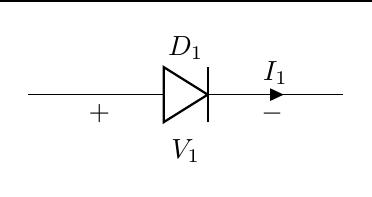
\begin{tikzpicture}[american voltages]
        \draw (0, 0) to[D=$D_1$, v=$V_1$, i=$I_1$] (40mm, 0);
    \end{tikzpicture}
    \caption{The first figure example. This is a diode.}
    \label{fig1}
\end{figure}

\lipsum[4-7]

\begin{figure}[h]
    \centering
    \smartdiagram[circular diagram:clockwise]{Edit,
      pdf\LaTeX, Bib\TeX/ biber, make\-index, pdf\LaTeX}
    \caption{This is the second figure. This figure shows an example of a flowchart.}
    \label{fig2}
\end{figure}

\lipsum[15]

\subsection{Another Subsection Test}
\lipsum[1-5]

\begin{table}[h]
    \centering
    \caption{The second test table}
    \begin{tabular}{|c||c|c|}
        \hline
        \bfseries Name & \bfseries Category \#1 & \bfseries Category \#2 \\\hline\hline
        Testname 1 & Item 1.1 & Item 1.2\\\hline
        Testname 2 & Item 2.1 & Item 2.2\\\hline
        Testname 3 & Item 3.1 & Item 3.2\\\hline
    \end{tabular}
    \label{tab2}
\end{table}

\lipsum[6]

\chapter{Third Chapter Name}
\section{Chapter Three Section One}
\subsection{Chater Three Section One Subsection One}
\lipsum[2-5]
\subsubsection{Subsubsection One}
\lipsum[12-15]

\begin{figure}[h]
    \centering
    \smartdiagram[priority descriptive diagram]{
      Develop a document structure,
      Choose a document class,
      Select suitable packages,
      Setup the document preamble,
      Write your document,
      Finetune the layout}
      
    \caption{This is the third figure example. This is another smartdiagram with different style.}
    \label{fig3}
\end{figure}

\lipsum[16-18]

\begin{figure}[h]
    \centering
    \includegraphics[width=.3\textwidth]{Images/afghan_girl.jpg}
    \caption{The well known ``Afghan Girl". In courtesy of Sharbat Gula, National Geographic Magazine.}
    \label{fig4}
\end{figure}

\lipsum[19-20]
\subsubsection{Subsubsection Two}
\lipsum[14-17]
\subsection{Chapter Three Section One Subsection Two}
\lipsum[15-20]
\subsection{Chapter Three Subsection Two}
\lipsum[10-15]

\chapter{Fourth chapter name}
\section{Section Four by One}
\lipsum[1-7]
\section{Section Four by Two}
\lipsum[8-12]

\begin{table}[h]
    \centering
    \caption{The third test table}
    \begin{tabular}{|c||c|c|}
        \hline
        \bfseries Name & \bfseries Category \#1 & \bfseries Category \#2 \\\hline\hline
        Testname 1 & Item 1.1 & Item 1.2\\\hline
        Testname 2 & Item 2.1 & Item 2.2\\\hline
        Testname 3 & Item 3.1 & Item 3.2\\\hline
    \end{tabular}
    \label{tab3}
\end{table}

\lipsum[30-32]

\begin{table}[h]
    \centering
    \caption{The fourth test table}
    \begin{tabular}{|c||c|c|}
        \hline
        \bfseries Name & \bfseries Category \#1 & \bfseries Category \#2 \\\hline\hline
        Testname 1 & Item 1.1 & Item 1.2\\\hline
        Testname 2 & Item 2.1 & Item 2.2\\\hline
        Testname 3 & Item 3.1 & Item 3.2\\\hline
    \end{tabular}
    \label{tab4}
\end{table}

\lipsum[13-15]

\chapter{This chapter introduces how to use some functionality}

In this chapter, reader may find how to use BibTeX (in Section \ref{bibtexsec}) and referencing on equations, figures and tables (Section \ref{referencesec}).

\section{How to Use BibTeX}

\label{bibtexsec}

Bib\TeX~allows an easy-to-master structure in terms of reference manipulation when using \LaTeX. The file in the main directory having the extension \texttt{.bib} is the main place that we ought to input all the references in Bib\TeX~format. The format is commonly accessible when we need to cite an article, proceeding etc. on the paper's website. However, many types of documents cited may not have a certain format. Hence, using the examples in ``\texttt{references.bib}" file is strongly recommended.

\subsection{BibTeX Examples}

In this sentence, the article in \cite{article_example} is cited. When you add your reference to the \texttt{references.bib} file, the cited references will automatically be added to the {\bfseries REFERENCES} section. After citing multiple references, they are sorted automatically by the first appearance in the document and numbered accordingly.

Let us add another citation of a book in \cite{book_example}. Multiple citations \cite{booklet_example, inbook_example} of a booklet and a book part will be printed out like in this sentence after compiling. Multiple citations should not be manually added, but they could be separated by commas as the arguments of \texttt{\textbackslash cite\{$\cdots$\}}. A collection part \cite{incollection_example}, a proceeding part \cite{inproceedings_example} and a manual \cite{manual_example} are cited as shown. The references of a master's thesis, a miscellaneous document, a PhD thesis, a proceeding, a tech report, and an unpublished publication are as shown in \cite{mscthesis_example, misc_example, phdthesis_example, proceedings_example, techreport_example, unpublished_example}.

\section{References to Equations, Figures and Tables}

\label{referencesec}

Composing and compiling an equation in \LaTeX is very simple. One may consider checking online resources to get used to equation composing using \LaTeX. Furthermore, using some online tools to generate equations from inline expressions or by using visual editors is also possible. Let us generate a comparably complex equation with unusual symbols. For example, the following is the definition of Hamming Distance.

\begin{equation}
    d_H(\pmb{x}, \pmb{y}) = \sum_{i=1}^{N} x_i \oplus y_,
    \label{hamming distance}
\end{equation}

where $x$, $y$, $N$, and $d_H$ corresponds to the first sequence, the second sequence, the bloc length and the Hamming Distance. The operation $\oplus$ denotes the binary XOR operation.

We can reference to the Equation~\ref{hamming distance} as shown. Also, figures and tables like Figure~\ref{fig1} and Table~\ref{fig3} can be referenced in the same manner.

Another way to represent equations are aligning. For example, the parametric equation

\begin{align*}
    x &= 5\sin^3(t)\\\nonumber
    y &= 4\cos(t)-1.3\cos(2t)-0.6\cos(3t)-0.2\cos(4t)
\end{align*}

will produce a mathematical heart. But, I preferred not to reference to it. Hence, I suppressed equation numbering by putting an asterisk (*) after the \texttt{align} command.

Let us check the following equations.

\begin{align}
    y_1&=x^2+3x+4 \label{eqfirstrow}\\
    y_2&=x^3+x^2+x+0.9\nonumber \\
    y_3&=x^2+\sqrt{x} \label{eqthirdrow}
\end{align}

I suppressed the second line as I only reference to the Equation~\ref{eqfirstrow} and Equation~\ref{eqthirdrow}.

\chapter{Conclusion}
\section{Conclusion Test Section}
\lipsum[1-10]
\section{Recommendations for Future Works}
\lipsum[11-18]

\newpage
\addcontentsline{toc}{subparagraph}{REFERENCES}
\renewcommand{\bibname}{\normalsize REFERENCES}
\bibliographystyle{IEEEtran}
\bibliography{references}

\appendix
\addcontentsline{toc}{paragraph}{APPENDICES}
\chapter{THE FIRST APPENDIX}
\lipsum[1-3]
\chapter{THE SECOND APPENDIX}
\section{Appendix Two Section one}
\lipsum[1-2]
\section{Appendix Two Section Two}
\lipsum[3-5]

\label{LastPageLabel}
\end{document}
